\documentclass{article}
\usepackage[utf8]{inputenc}
\usepackage{authblk}
\usepackage{graphicx}

\title{EEG2fMRI: Cross-Modal Synthesis for Functional Neuroimaging}
\author{Paul Bricman}
\author{Jelmer Borst}
\affil{University of Groningen}
\date{July 2021}

\begin{document}

\maketitle

\begin{abstract}
    Functional neuroimaging techniques are essential in advancing research in neuroscience. However, existing techniques require researchers to either compromise on spatial resolution, temporal resolution, cost, or portability. We attempt to model the  mapping between concurrent EEG and fMRI recordings using various machine learning architectures, in order to combine the complementary qualities of the two modalities. The trained model is then able to reconstruct simultaneous fMRI data solely from EEG data. Although initial results in a within-subject regime are promising, the limited quantity of multi-modal recordings currently available appears to be a major obstacle in generalizing to new subjects.
\end{abstract}

\section{Introduction}

Neural activity is central to investigating cognition. In cognitive neuroscience, it has been employed to study the neural correlates of many cognitive functions, such as perception, attention, and memory. In cognitive modelling, neural activity has been used to inform the development of a wide range of cognitive architectures. In clinical neuroscience, it has been employed for investigating, diagnosing, and ameliorating a wide range of neurological conditions \cite{n_functional_2015}.

The increased relevance of neural activity in cognitive science prompted the development of a large number of functional neuroimaging techniques. These techniques can be effectively described in terms of spatial resolution, temporal resolution (sampling rate), and portability. The most widely used functional neuroimaging techniques are EEG and fMRI. EEG scanners consist of arrays of electrodes placed directly on the user's scalp. They are extremely portable and have high temporal resolution. However, such scanners can only detect neural activity after first being filtered by the skull, leading to a major decrease in spatial resolution. Conversely, fMRI is based on electromagnetic waves which easily penetrate the skull. Therefore, it has high spatial resolution, but is lacking in most other aspects. Compared to EEG, it is hundreds of times more expensive and thousands of times slower. Moreover, it is virtually unmovable by its user.

Given the lack of techniques which individually exhibit high overall performance, there have been numerous attempts to integrate their complementary qualities by using multiple techniques simultaneously. EEG-informed fMRI, fMRI-informed EEG, and neurogenerative modelling are all methods of integrating data from simultaneous EEG and fMRI recordings. However, these methods require extensive access to both neuroimaging techniques involved and are limited to niched applications \cite{huster_methods_2012}. 

Besides multi-modal functional neuroimaging, investigators have also proposed uni-modal synthesis as a method of augmenting neuroimaging techniques. This consists of conditionally synthetizing novel data based on previous data collected through the same modality. This method has been found to increase performance in downstream machine learning classifiers based on fMRI data \cite{zhuang_fmri_2019}.

In addition to uni-modal synthesis, investigators have also proposed cross-modal synthesis for augmenting neuroimaging techniques. This consists of reconstructing data collected through a target modality based on data collected through a distinct source modality, by exploiting the inherent relation between them. In a setting where both source and target modalities are available, this task might have limited utility. However, the value of cross-modal synthesis comes from settings where only one modality is available. In such settings, existing data can be used to approximate data collected through the unavailable modality. Unfortunately, this approach has largely been used for augmenting structural neuroimaging, with limited analogous efforts for functional neuroimaging \cite{yi_generative_2019}.

Despite the major demand for high-performance functional neuroimaging and the success of cross-modal synthesis for structural neuroimaging, limited attention has been given to cross-modal synthesis for functional neuroimaging. The purpose of the current work is to explore the feasibility of this method. This comes as a natural extension to the growing collection of functional neuroimaging augmentation methods.

\section{Task}

The task of modelling the relation between two functional neuroimaging modalities can be addressed through at least three different approaches. This decision is mainly based on data availablility.

First, if simultaneous multi-modal recordings are available, supervised learning can be employed to model the mapping between the two domains based on paired samples. Unfortunately, the constraint of physical compatibility greatly restricts the pairs of modalities which can be investigated. For instance, MR-compatible EEG scanners have to be manufactured with special materials, in order to avoid physical injury during EEG-fMRI operation. Fortunately, the development of multi-modal methods of data integration has highlighted multiple candidate pairs of modalities for simultaneous recording \cite{yi_generative_2019}.

Second, if simultaneous multi-modal recordings are not available, but separate recordings of similar neural states with different modalities are available (i.e. two separate recording sessions based on the same task but using different techniques), semi-supervised learning can be used to model the mapping through a task-related signal. This is analogous to the task of machine translation, which is often based on sample pairing through a cross-lingual signal \cite{zhang_neural_2020}.

Third, if the quantity of such recordings is limited, unsupervised learning can be used to learn the mapping by learning to align the latent spaces associated with the two modalities. This is analogous to machine translation where no paired multilingual corpora exist \cite{lample_phrase-based_2018}. The following sections focus on supervised cross-modal synthesis, as the setup it requires is the most straight-forward.

The suitability of EEG-fMRI as a candidate pair for supervised cross-modal synthesis is supported by the established practices of multi-modal neuroimaging using EEG-fMRI \cite{huster_methods_2012}. These practices are the result of physical compatibility and the presence of complementary qualities. Not only are EEG and fMRI compatible and complementary, but their results are also strongly correlated \cite{ostwald_eeg-fmri_2009}. The correlation occurs because both techniques can be used to record the same neural activity, albeit in different ways.

\section{Data}

We used a dataset from a multi-modal neuroimaging study which involved visual and auditory oddball tasks \cite{noauthor_auditory_nodate}. The reason we chose this dataset, among other multi-modal neuroimaging ones, was that visual and auditory areas might be easier for the model to distinguish compared to more distributed networks of regions. Based on this dataset, we derived individual samples with the following structure. The input part of a data point consists of a 30-second-long EEG recording across 34 electrodes at 1000Hz. This data resembles 34 parallel time series unfolding across 30 seconds (Fig. \ref{fig:eeg}). Each time series originates from a certain electrode placed in a certain place on the subject's scalp.

\begin{figure}[h]
    \centering
    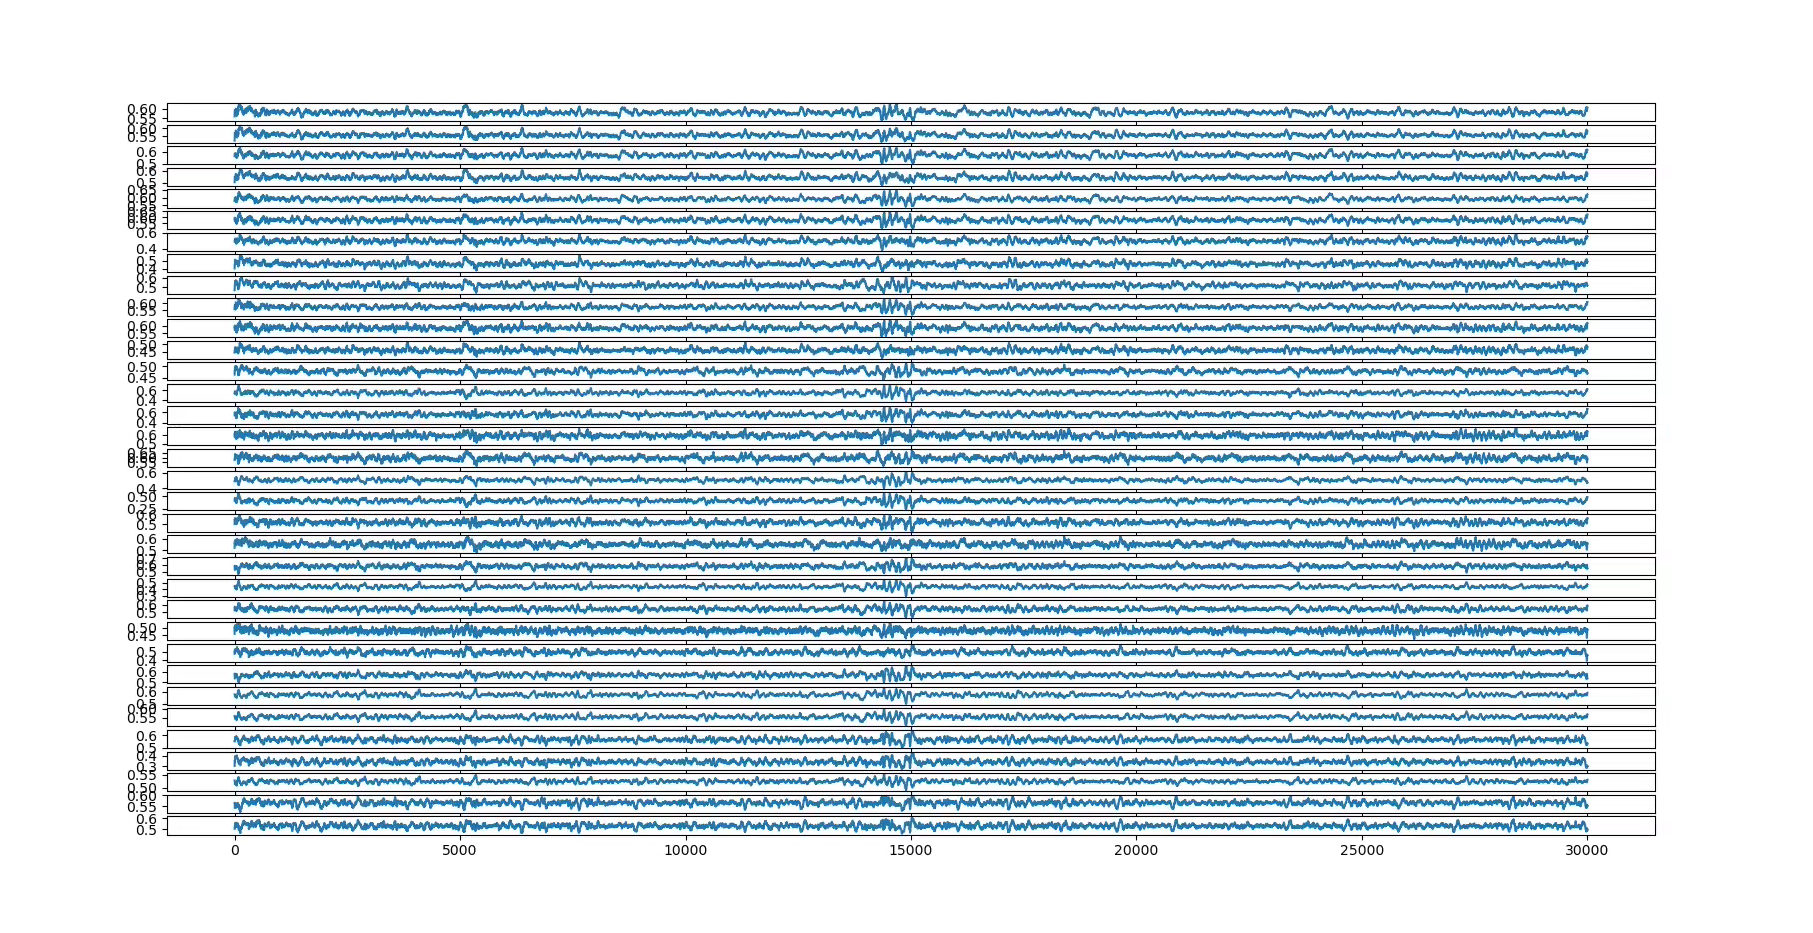
\includegraphics[width=\textwidth]{eeg.png}
    \caption{An input sample consisting of 34 parallel EEG signals}
    \label{fig:eeg}
\end{figure}

The output part of a data point consists of a three-dimensional tensor of shape 53x63x52 which depicts the 3D "picture" of the subject's brain obtained through fMRI at the time roughly corresponding to the end of the EEG recording.

For the input part of a data point, the recording length of 30 seconds has been chosen for the following reason. fMRI does not record neural activity per se, but blood oxygen levels, the BOLD response, which is a reasonable proxy for neural activity. However, the BOLD response is not an immediate one-to-one reflection of neural activity, but the result of a convolution between neural activity and a response curve informed by brain physiology, the BOLD response curve \cite{noauthor_functional_1993}. This is conceptually similar to how food consumption isn't instantly reflected in blood sugar levels, but reflects the result of a convolution informed by metabolism. In the case of fMRI, recordings at any given time are influenced by neural activity which occured roughly during the previous 30 seconds. Therefore, 30 seconds of EEG are paired with one fMRI scan obtained at the end of the EEG recording, forming a data point. In contrast, EEG data itself closely reflects neural activity unfolding at that exact time of recording (albeit with very poor spatial resolution).

The raw original dataset is structured as follows. There are 16 subjects (after excluding one whose data was corrupted), each undergoing 6 blocks of an oddball task. Each block contains 170 fMRI scans, obtained sequentially, at a frequency of 0.5 Hz (for a total of 340 seconds per block). Each block also contains EEG data, recorded constantly at 1000Hz for the entire duration of the block. From these longer sequences of data, we are extracting data points in the way described previously. However, we're discarding the first few fMRI scans obtained before 30 seconds of EEG managed to accumulate beforehand. This means that ~155 samples are derived per block, which translates to 930 per subject, which translates to 14880 in total.

In terms of preprocessing, EEG data was normalized per subject and per channel. The reasoning behind this was to remove influences of electrodes being placed in slightly different locations across subjects. The preprocessing pipeline for fMRI is more complex, consisting of: motion correction, slice time correction, registration, normalization, and smoothing. Additionally, each tensor obtained through a fMRI scan has been masked in order to only contain non-zero values at locations which are known to contain white and gray matter. All these preprocessing stages where used to increase the signal-to-noise ration in both EEG and fMRI, limiting the influence of subject-specific particularities on the data so that the mapping would be performed as effectively as possible.

\section{Models}

A wide range of model architectures have been employed for learning the EEG-fMRI mapping. Initially, dense fully-connected networks were tasked with encoding the entire flattened EEG data of one sample into one embedding of lower dimensionality through a linear layer. This embedding would be further routed through subsequent linear layers. The last layer would contain a number of neurons equal to the number of voxels present in the fMRI scans, so that they could be trained to directly predict the voxel-level activity.

However, the initial projection of the entire EEG data of one sample to a space with lower dimensionality would require a high number of parameters to be learned. Additionally, one could assume that the separate EEG channels would possess similar information, and that similar models could be useful for deriving information from different EEG channels. In light of this, the initial layer which embedded the entire EEG data of a sample has been turned into a less complex layer which embedded one EEG channel at a time. This subnetwork would be used to derive embeddings for each of the 34 EEG channels, while using and learning the same weights. This Siamese-network design choice helps reduce the number of trainable parameters \cite{bromley_signature_nodate}.

However, the model still performed poorly with this architecture, prompting us to speculate that the dense fully-connected architecture is not expressive enough to learn the EEG-fMRI mapping. Therefore, we turned the one-channel fully-connected embedding network into a series of convolutional layers, which presumably extracted more relevant features from the time series associated with each EEG channel. The embeddings from all EEG channels would get concatenated before being piped through subsequent linear layers, ending in an output layer identical to the previous one.

Extending the complexity of the model further following the limited success in learning the mapping resulted in employing a transformer architecture \cite{vaswani_attention_2017}. The EEG data associated with one individual data point was structured into a sequence of EEG channels. Each one-channel EEG recordings would be embedded as before using a layer shared across channels \cite{dosovitskiy_image_2020}. However, with the transformer architecture, the channel embeddings would be treated as a sequence, rather than being concatenated. Additionally, the fMRI data cube associated with a sample would also be structured as a sequence of slices. Using the transformer architecture, the task of mapping EEG data to simultaneous fMRI data resembles a sequence-to-sequence transduction task, mapping a sequence of EEG channels to a sequence of fMRI slices.

The reasoning behind employing a transformer architecture was the following. When generating a slice as output, the model could attend to previously generated slices. This is likely to improve performance, as the activity in nearby slices is highly correlated. Large brain regions and vast networks operate together, making the generation of a new slice dependent on previous ones. Additionally, when generating a new slice, the transformer model could attend to any EEG channel embedding, making use of the ones providing the most useful information. Both sinusoidal and learned positional encodings have been used. We expected learned positional encodings to eventually match the electrode positions after training, similar to how learned patch embeddings for image classification converge to a grid \cite{dosovitskiy_image_2020}.

\section{Results}

In a setting in which the time course normalization is absent and the entire dataset is randomly shuffled into training data and testing data, all models except for the ones based on the transformer architecture manage to converge to non-trivial solutions on testing data. The predicted fMRI scans are more similar to the ground truth scans than both a global average scan and an subject-level  average scan, indicating that the models avoided the failure modes of resorting to outputing global or subject-level average scans regardless of EEG input.

In contrast, in a setting in which either time course normalization is introduced or the train-test split policy is based on entirely leaving out one subject during training, no models manage to converge to non-trivial solutions on the testing data. In multiple configurations, the models either learn to output an average fMRI scan or learn to output a completely unrelated scan which is slightly influenced by EEG input.

\section{Discussion}

In this project we attempted to learn the mapping between EEG data and concurrent fMRI data through a host of machine learning models. The task proved to be particularly challenging, especially in a between-subject regime, where the model is tested on data originating from a subject not considered at all during training. This might indicate that subject-specific information is necessary for the model to be able to conduct the EEG-fMRI mapping. Anatomical particularities specific to the subject might make generalization to new subjects difficult. In contrast, in a within-subject regime, most models perform well. However, the within-subject regime defeats the purpose of attempting the mapping, given that both neuroimaging methods involved are accessible.

The difficulty in generalization might have been mainly caused by the limited size of the dataset considered, in the order of thousands. Deep learning models are known to require a large number of samples in order to generalize. Data augmentation methods such as performing random vertical shifts of the EEG signals and adding random noise had limited impact on generalization. The quantity of multimodal EEG-fMRI recordings remains a challenge for such a supervised approach to the cross-modal mapping. This challenge is likely caused by the difficulty in running experiments which not only make use of expensive fMRI machines, but which require additional expertise in EEG-fMRI compatibility and MR-compatible EEG headsets \cite{calhas_eeg_2020}.

This state of affairs suggests that self-supervised approaches might be more suitable candidates for attempting the EEG-fMRI mapping. Large amounts of uni-modal EEG data are available, and the same is true for uni-modal fMRI data, although to a lesser extent. Approaches which incorporate both types of uni-modal data might be more effective than ones which incorporate smaller multi-modal datasets. This resembles the shift towards unsupervised methods of machine translation where sufficiently large paired corpora do not exist.

Generating synthetic data based on an existing multi-modal dataset might be another way of tackling the issue of limited samples. While generative models have been successfully used to synthesize uni-modal data, the same cannot be said about synchronous multi-modal data. An even simpler solution to the problem might be to join all publicly available multi-modal EEG-fMRI datasets into one larger one, and learn the mapping based on the resulting dataset. However, those few datasets available which match the criterion typically use scanners with wildly different specifications. From the number of EEG channels used to the sampling frequency of the fMRI scanner, it might be challenging to merge those into a generic dataset.

Learning the mapping between simultaneous EEG and fMRI recordings remains an open challenge which might enable powerful tools for neuroscientists of various specializations. The limited quantity of data currently available appears to be a major obstacle in solving this task.

\bibliographystyle{plain}
\bibliography{eeg2fmri}

\end{document}
